\begin{figure}[h!]
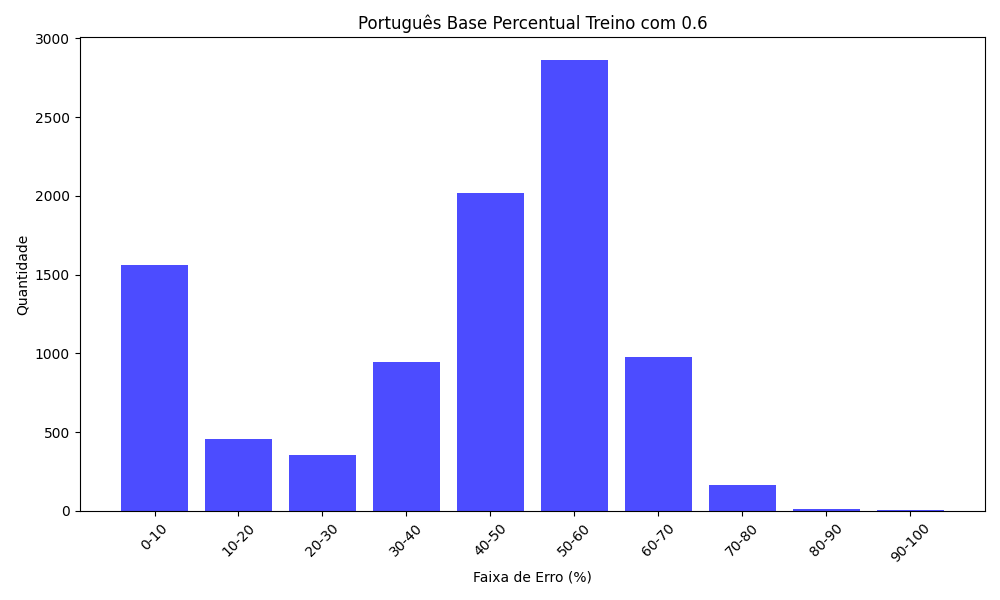
\includegraphics[width=\textwidth]{img/grafsPort/Português Base Percentual Treino com 0.6_quantidade.png}
\caption{Quantidade de respostas por faixas de erro percentual dos testes com 40\% do \textit{dataset Galhardi} (Português) usando o Modelo \textit{BERTimbau Base})}\label{figure:44}
\end{figure}

\begin{figure}[h!]
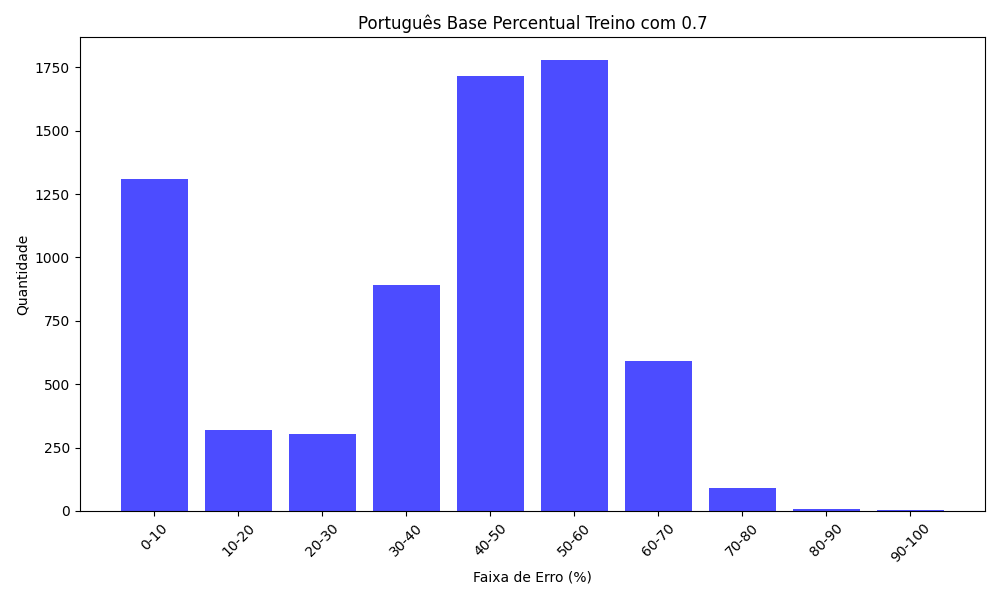
\includegraphics[width=\textwidth]{img/grafsPort/Português Base Percentual Treino com 0.7_quantidade.png}
\caption{Quantidade de respostas por faixas de erro percentual dos testes com 30\% do \textit{dataset Galhardi} (Português) usando o Modelo \textit{BERTimbau Base})}\label{figure:45}
\end{figure}

\begin{figure}[h!]
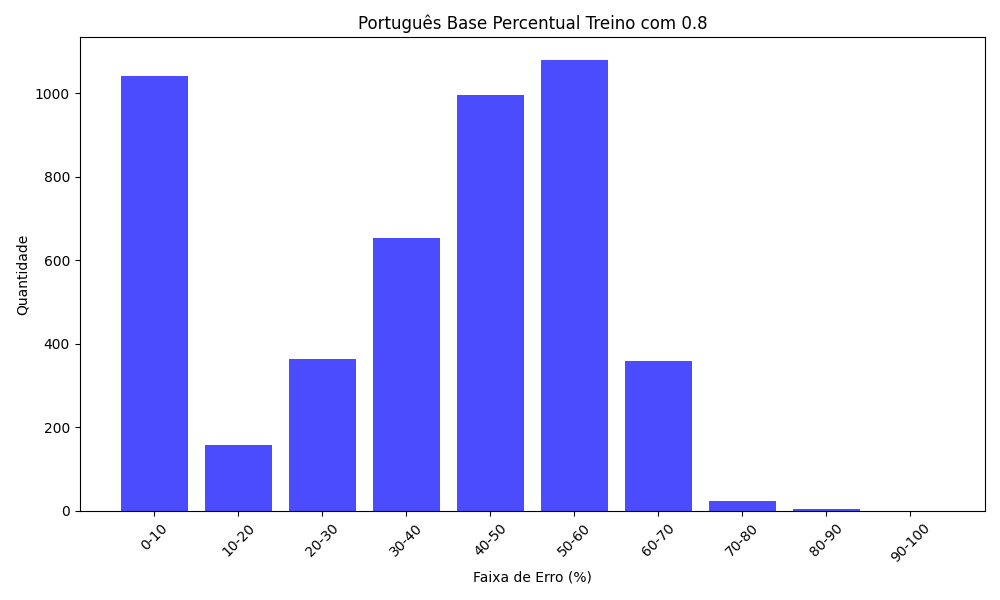
\includegraphics[width=\textwidth]{img/grafsPort/Português Base Percentual Treino com 0.8_quantidade.png}
\caption{Quantidade de respostas por faixas de erro percentual dos testes com 20\% do \textit{dataset Galhardi} (Português) usando o Modelo \textit{BERTimbau Base})}\label{figure:46}
\end{figure}

\begin{figure}[h!]
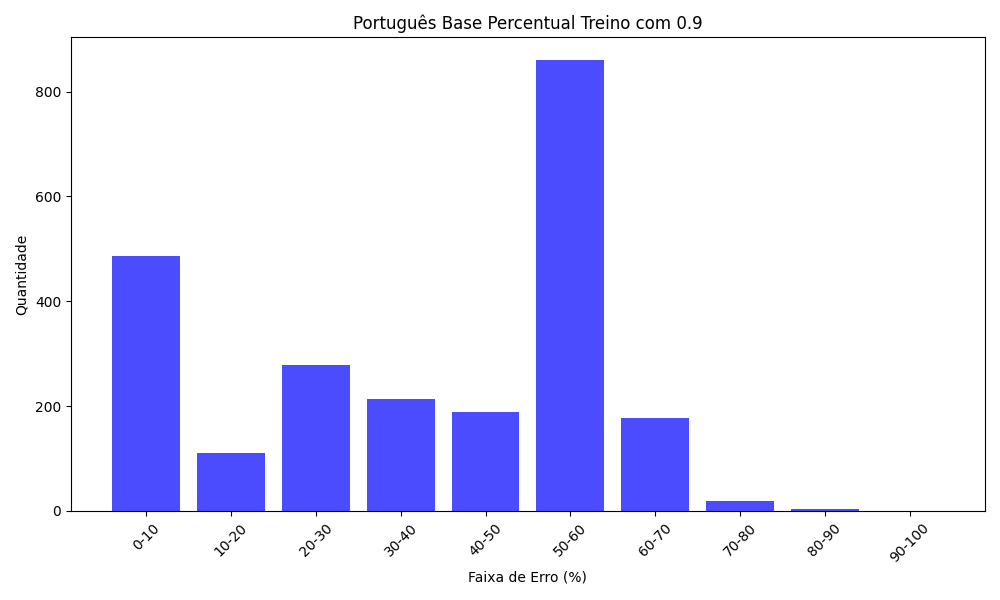
\includegraphics[width=\textwidth]{img/grafsPort/Português Base Percentual Treino com 0.9_quantidade.png}
\caption{Quantidade de respostas por faixas de erro percentual dos testes com 10\% do \textit{dataset Galhardi} (Português) usando o Modelo \textit{BERTimbau Base})}\label{figure:47}
\end{figure}